\documentclass[doktyp=marbeit,fontsize=11pt]{TUBAFarbeiten}

% packages
\usepackage{amsmath}
\usepackage[ngerman]{babel}
\usepackage{blindtext}
\usepackage{caption}
\usepackage{calc}
\usepackage{cite}
\usepackage{enumitem}
%\usepackage{float} % for better picture
\usepackage[T1]{fontenc}
\usepackage{floatrow} % rows of table and pictures
\usepackage{graphicx}
\usepackage{gensymb}
\usepackage[utf8]{inputenc}
\usepackage{makeidx}
\usepackage[fleqn]{mathtools} % mathtools und links buendig machen
\usepackage{multirow} % tabellen mit mehreren zeilen pro zelle
\usepackage{subcaption}
\usepackage{subscript} % tief stellen
%\usepackage[square]{natbib}

\DeclarePairedDelimiter{\abs}{\lVert}{\rVert} % definiere absoluten betrag

% tubaf zeugs
\TUBAFFakultaet{Fakultät für Mathematik und Informatik}
\TUBAFInstitut{Institut für Informatik}
\TUBAFLehrstuhl{Lehrstuhl für virtuelle Realität und Robotik}
\TUBAFTitel{Sensor Localization of Range Data using a Feature based Registration}
\TUBAFBetreuer{Prof. Dr. Bernhard Jung}
\TUBAFKorrektor{Dipl-Ing. Mark Sastuba}
\TUBAFAutor[J. Toth]{Jonas Toth}
\TUBAFStudiengang{Angewandte Informatik}
\TUBAFMatrikel{57319}
%\TUBAFAnmeldeDatum[2017-02-8]{8. Februar 2017}
\TUBAFDatum[2019-09-25]{25. September 2019}

%\setcounter{tocdepth}{2}
%\setcounter{secnumdepth}{3}

\makeindex

% start the content
\begin{document}

\maketitle
% \TUBAFErklaerungsseite
% \tableofcontents

\newpage

The dominant method to register pointclouds with pointclouds or depth
images is the use of a variant of the ICP (Iterative Closest Points)
algorithm. Even though there are many different approaches to ICP, it has
some common problems. The algorithm requires a good initial
transformation. Pointclouds with order-of-magnitude different
resolutions can produce unstable results. Convergence might require many
iterative steps and can not be predicted. Each of these iterative steps
is computationally expensive and does not scale very well to massive
datasets.

All these apsects give opportunity for a better solution to the problem
of registering depth images, e.g.~from the Kinect-v2, to existing
high-resolution pointclouds.

\subsection{Approach}\label{approach}

\subsubsection{Preprocessing of range Data}\label{preprocessing-of-range-data}

\begin{figure}[H]
    \centering
    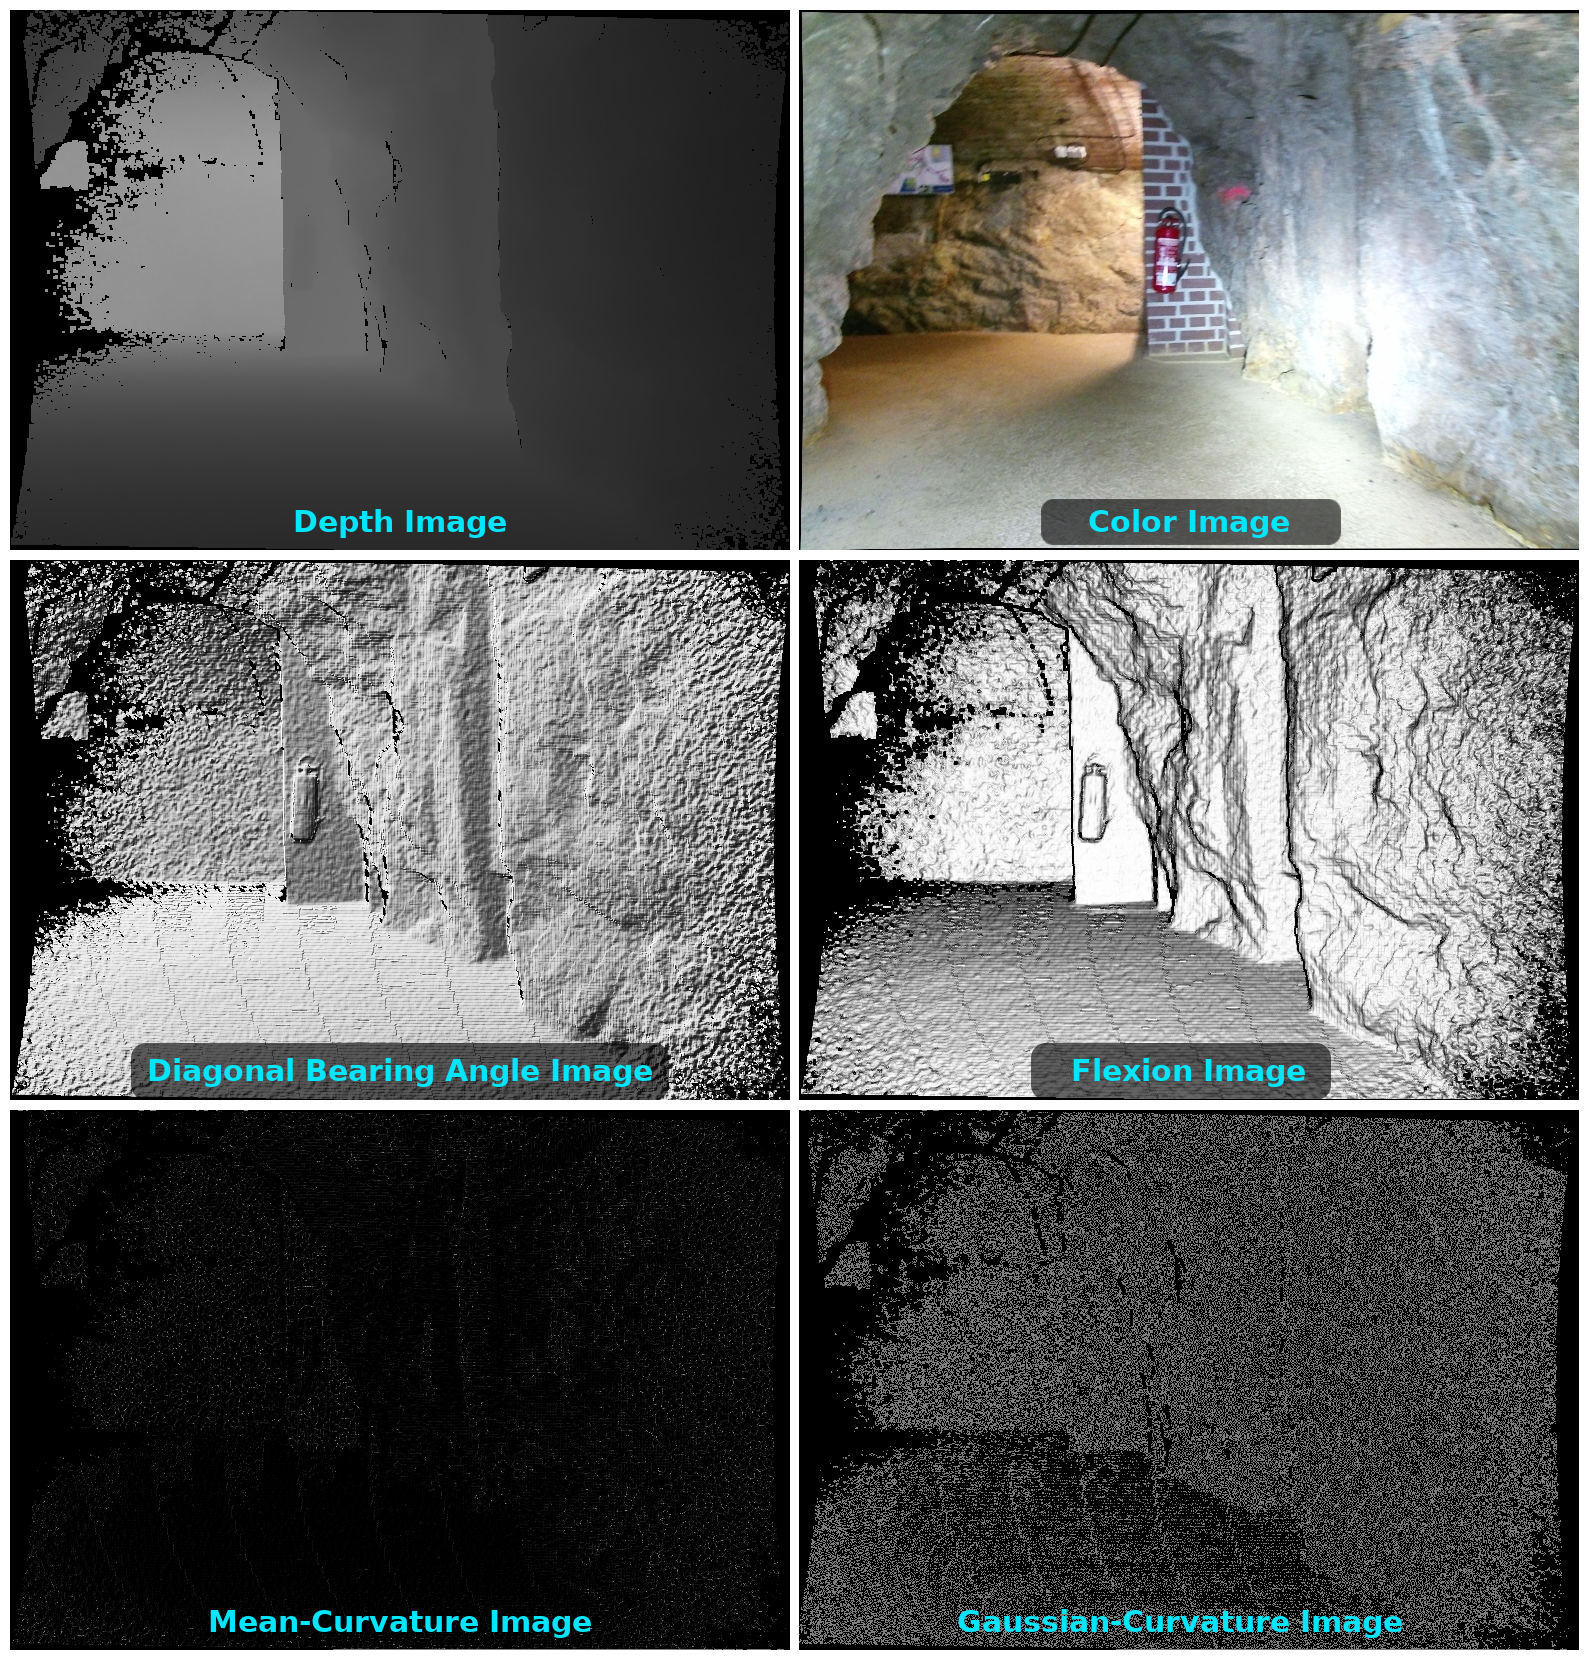
\includegraphics[width=0.9\textwidth]{images/collage_v2.png}
    \caption{Overview of possible Feature-Images from a (in this image scaled) depth image}
\end{figure}

Instead of registering the depth images based on single points and their
distance to other points, this thesis develops a new framework to use
existing image features like SIFT and SURF to calculate the
transformation between pointcloud and depth image. Both, the pointcloud
and the depth image, are first converted to a gray-scale image. Instead
of just using the distance present in depth-images these new images
encode the local geometry, called feature-images.

Existing literature proposes Bearing Angle images were each pixel is the
angle between the current point, the optical center and the previous
point. Part of this thesis is the development of a new calculation
method named flexion images.

Each pixel of a flexion image is dot-product of the local normal
calculated from horizontal and vertical neighbouring pixel with the
normal calculated with the diagonal neighbours.

The dot-product then results in the angle between both of these vectors.
The smaller the dot-product gets, the higher is the local flexion of the
surface. This local property of the geometry then results in visual
features detectable with classical feature detectors and descriptors like
SIFT.

Futhermore, the conversion of range data to feature images can be done
for laserscans and virtual laserscans, e.g.~from a reconstructed mesh,
too.

\subsubsection{Transformation calculation}\label{transformation-calculation}

Starting with the feature image, a visual localization pipeline is
established that works solely on omnidirectional data, thus is general
enough to utilize a wide range of sensors and camera models.

The full workflow of the pipeline is as follows:

\begin{enumerate}
\item Omnidirectional images are mapped onto a cubemap to reduce distortion,
  the feature images are calculated for both the data to localize,
  e.g.~Kinect depth image and the reference data, e.g.~terrestrial
  laserscans.
\item Visual Features are detected and matched between the sensor to
  localize and the reference data.
\item Classical RANSAC performs the stable calculation of the
  Essential matrix that is then decomposed into rotation and translation.
\item The resulting rotation and translation is optimized. The objective
  function is the distance of the detected features to the epipolar
  lines.
\item The unscaled translation is scaled with the depth data from the sensor
  input. This scaling can be done both with the input depth sensor and
  the reference data. The resulting difference is again subject to
  optimization.
\end{enumerate}

The result is the pose of the camera relative to the registered image as well as an error of the pose.

\subsection{Novelity}\label{novelity}

The idea to use optical features for multimodal sensor registration is
not new and goes back to Scaramuzza's approach to calibrate a
laserscanner to an optical camera. To the best knowledge of the author
only bearing angle images were used though.

Bearing angle images do come with some issues. They encode only the
relationship of two neighbouring points. Therefore, they are not
invariant to rotation. It is possible to calculate the bearing angle in
all eight bearing directions (horizontal, vertical, diagonal, antidiagonal in
both directions). This results to higher computational costs, especially
for the feature detection and matching pipeline.

This is the reason this work proposes different feature images that all
encode local geometry as a scalar value, gaussian curvature, mean
curvate and flexion as described above. These feature images are
compared to bearing angles. Flexion images are expected to perform the best
as they give the best visual structure.

If the proposed localization pipeline does work as wished it gives a new
intermodal approach to localization and visual odometry.

Futhermore, it allows to apply algorithms and approaches from the
classical visual feature-world to depth sensors that became widely
available in robotic operations.
 
% \input{verzeichnisse/bezeichnungen.tex}
% \newpage
% 
% \input{einfuehrung/content.tex}
% \newpage
% \input{grundlagen/content.tex}
% \newpage
% \input{modelle/content.tex}
% \newpage
% \input{intrinsic/content.tex}
% \newpage
% \input{extrinsic/content.tex}
% \newpage
% \input{evaluierung/content.tex}
% \newpage
% \input{fazit/content.tex}
% \newpage
% 
% \appendix
% \input{anhang/content}
% \newpage
% 
% \bibliography{verzeichnisse/literatur}
% \bibliographystyle{plain}
% 
% \listoftables
% \listoffigures
% \newpage

%\renewcommand{\indexname}{Stichwortverzeichnis}
%\addcontentsline{toc}{section}{Stichwortverzeichnis}
% \printindex

\end{document}
